% 18W MOSFET amplifier, with npn transistor.
% Author: Ramón Jaramillo.
\documentclass[margin=10pt]{standalone}
\usepackage[siunitx]{circuitikz}
\begin{document}
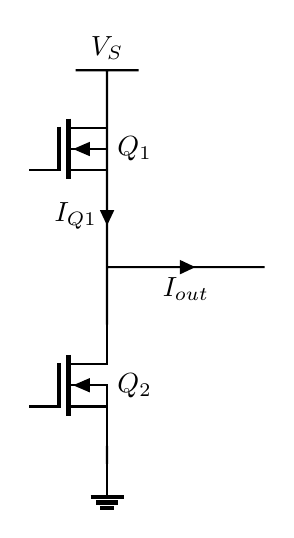
\begin{tikzpicture}[scale=2]
  \draw[color=black, thick]

    % Input and ground
    (4.8,4) to (5.2,4)
    (5,4)node[above]{$V_S$} to (5,3) 
    % Mosfet Transistors
    (5,3) to [Tnigfetd,n=mos1] (5,4)
    (5,3.4)  to [short, i_=$I_{Q1}$] (5,2.75)
    (mos1.B) node[anchor=west]{$Q_1$} % Labelling MOSFET Q2 Transistor
    (5,2.75)  to [short, i_=$I_{out}$] (6,2.75)
 
    (5,1.5) to [Tnigfetd,n=mos2] (5,2.5)
   % (5,0) to (mos2.S)
    (mos2.S)--(5,1.5)node[ground]{}
    (mos2.B) node[anchor=west]{$Q_2$} % Labelling MOSFET Q3 Transistor
    (mos1.S)--(mos2.D)
    ;
\end{tikzpicture}
\end{document}
